\section{Durchführung}
\label{sec:Durchfuehrung}

Bei dem Versuch kommen ein Lock-In-Verstärker, ein Oszilloskop, eine
LED und eine Photodiode zum Einsatz. Der Lock-In-Verstärker beinhaltet
einen Funktionsgenerator  mit 2 Ausgängen, einen Phasenschieber und einen
Rauschgenerator. Nachfolgend ist ein beschriftetes Bild des verwendeten Geräts
zu sehen:
\begin{figure}[H]
  \centering
  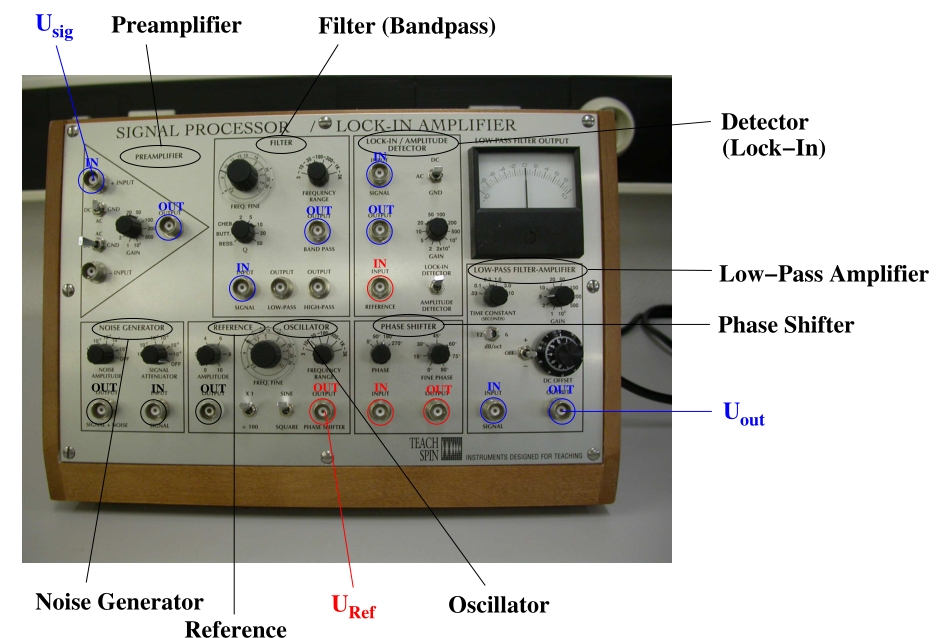
\includegraphics[keepaspectratio, width=0.6\textwidth]{geraet.png}
  \label{fig:gerät}
\end{figure}
Abb. aus : \cite[3]{Anleitung}


\subsection{Funktionsgenerator}
Der erste Teil des Versuches befasst sich mit der Funktionsweise des Geräts.
Dafür werden die Spannungen an beiden Ausgänge des Funktionsgenerators einzeln
vermessen um festzustellen welcher Ausgang eine regelbare Spannungsamplitude
generiert.

\subsection{Mischen der Signale}
In dem zweiten Versuchsabschnitt werden die beiden generierten Signale gemischt
und integriert. Dafür wird folgende Schaltung aufgebaut:

\begin{figure}
  \centering
  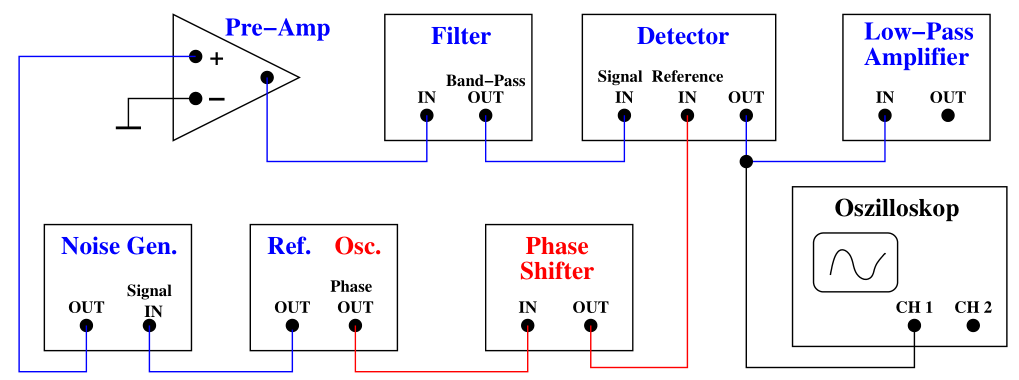
\includegraphics[keepaspectratio, width=0.6\textwidth]{Schaltung1.png}
  \label{fig:Schaltung1}
\end{figure}
Abb. aus: \cite[1]{Anleitung}\\

Der Rauschgenerator wird zunächst nicht verwendet (Rauschen auf off einstellen).
Die Signalspannung mit einer Frequenz von 1Khz und einer Amplitude von 1V
wird verstärkt und mit der
Referenzspannung gemischt. Gemessen werden die Ausgangsspannung $U_{out}$
sowie die am Tiefpaß
integrierte Ausgangsspannung für verschiedene Phasenverschiebungen $\phi$. Auf
diese
Weise wird die Phasenabhängigkeit der integrierten Spannung nachgewiesen.

\subsection{Rauschgenerator}
Für diesen Versuchsteil wird der Signalspannung ein Rauschen beigefügt. Dazu
wird der Rauschgenerator eingestellt und ein Rauschen erzeugt, dessen
Größenordnung um eine unter der des Signals liegt. Daraufhin werden alle
Messungen aus dem zweiten Versuchsteil wiederholt um die Ergebnisse mit den
unverrauschten Werten zu vergleichen.

\subsection{LED und Photodiode}
Im letzten Abschnitt wird die aus den anderen Versuchsteilen bekannte Schaltung
leicht abgewandelt. Anstatt die Signalspannung direkt zu vermessen wird mit ihr
eine LED betrieben.Das von der LED ausgestrahlte Licht wird von einer Photodiode
im Abstand $r$ vermessen. Die Photodiode ist an den Eingang des Verstärkers
angeschlossen. Die Spannung der Diode wird
- nachdem sie den Bandpass passiert hat - mit der
Referenzspannung gemischt und die resultierende Spannung an
Oszilloskop und Tiefpaß bestimmt.
